\begin{figure}[ht]
    \centering
  
    %======================
    % Program
    %======================
    \begin{minipage}[c]{\textwidth}
      \begin{lstlisting}[escapeinside={<@}{@>},aboveskip=0.1em,belowskip=0.1em]
      let x = if flip() <@\textcolor{purple}{then}@> 0.5 <@\textcolor{purple}{else}@> 1.5 in gaussian(0, <@\textcolor{red}{x}@>) <@\textcolor{orange}{<}@> 0.5
      \end{lstlisting}
    \end{minipage}
  
    \vspace{0.8em}
  
    %======================
    % Constraint graph
    %======================
    \begin{minipage}[c]{\textwidth}
        \centering
        \scalebox{0.58}{
        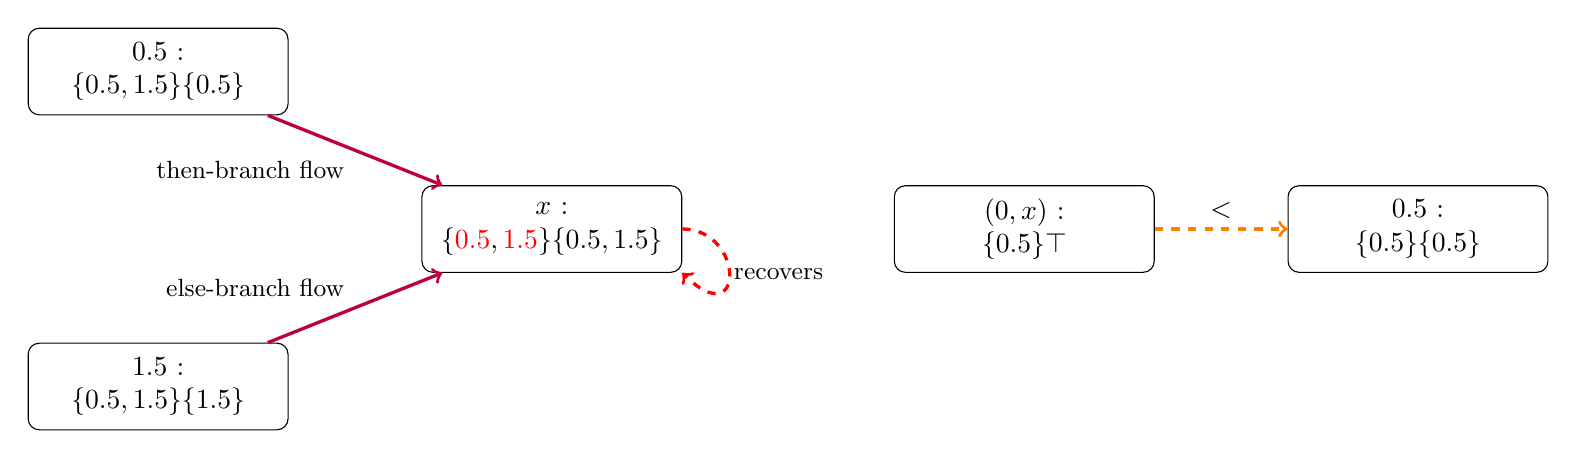
\begin{tikzpicture}[
            floatnode/.style={draw, rounded corners, minimum width=3.3cm, minimum height=1.1cm, align=center},
            flow/.style={->, very thick, draw=purple},
            constraintlt/.style={->, very thick, dashed, draw=orange}
        ]
        
        % ===== FLOAT VALUE NODES =====
        
        \node[floatnode] (v05) at (-6, 2) {
            0.5 : \\
            $\floattype{\{\cleq{0.5}, \cleq{1.5}\}}{\{0.5\}}$
        };
        
        \node[floatnode] (v15) at (-6, -2) {
            1.5 : \\
            $\floattype{\{\cleq{0.5}, \cleq{1.5}\}}{\{1.5\}}$
        };
        
        % ===== X NODE =====
        
        \node[floatnode] (x) at (-1, 0) {
            $x$ : \\
            $\floattype{\{\textcolor{red}{\cleq{0.5}}, \textcolor{red}{\cleq{1.5}}\}}{\{0.5,1.5\}}$
        };
        
        % ===== SINGLE GAUSSIAN NODE =====
        
        \node[floatnode] (g) at (5, 0) {
            $\gaussian(0, x)$ : \\
            $\floattype{\{\clt{0.5}\}}{\top}$
        };
        
        % ===== CONSTANT 0.5 NODE =====
        
        \node[floatnode] (c05) at (10, 0) {
            0.5 : \\
            $\floattype{\{\clt{0.5}\}}{\{0.5\}}$
        };
        
        % ===== DATA FLOW EDGES (match Step 1 placement style) =====
        
        \draw[flow] (v05) -- node[below left] {\small then-branch flow} (x);
        \draw[flow] (v15) -- node[above left] {\small else-branch flow} (x);
        
        % ===== SELF LOOP ON X WITH "recovers" =====
        
        \draw[flow, color=red, dashed, very thick]
            (x.east) .. controls +(0.8,0) and +(0.8,-0.8) ..
            node[right, text=black, inner sep=1pt] {\small recovers}
            (x.south east);
        
        % ===== GAUSSIAN TO CONSTANT LINE =====
        
        \draw[constraintlt] (g) -- node[above] {$<$} (c05);
        
        \end{tikzpicture}
        }
    \end{minipage}
  
    \caption{Constraint graph populated with float type information. As before, solid arrows represent data flow, and dashed arrows represent comparison constraints. Using $x$ as a Gaussian parameter induces a \emph{recovers} constraint, the red dashed self-loop, which ensures a unique discrete index for each value of $x$.}
    \label{fig:control-flow-distinguishes}
 \end{figure}